\chapter{HIL felépítése}

\section{Hardware felépítése}

A HIL szimulátor hardware nem más, mint egy interface elektronika a vezérlő hardware-ek és a szimulációt végző FPGA között. \Afigref{hw_architect} ábrán láthatóak a vezérést végző elemek. A HIL szimulátor feladata a bal oldali, Power Subsystemb blokkból érkező jelek előállítása, illetve a vezérlő jelek fogadása. Mivel a szimuláció során a PIB nem szükséges, ezért az MCB és a CCB kapcsolatát is a HIL elektronika biztosítja.

\todo[inline]{Blokkvázlat a HIL-ről}

\subsection{Tápegység}
A kártya $24 V$-os tápfeszültségre lett tervezve. Ebből egy Linear Technologies \emph{LT3845AEFE#PBF} szinkron buck tápegység vezérlő IC és a hozzá tartozó külső apparátus állítja aelő az $5 V$-os tápfeszültséget mind az FPGA mind pedig a CCB számára. A tápegység maximálisan $6 A$ terhelhetőségű, amely előser soknak tűnhet, de az FPGA fogyasztását jelentpsen befolyásolja a benne található firmware, így elképzelhető az kapacitás teljes felhasználása is, kis teljesítmény esetén edig hatékony tud maradni az ún. \emph{Burst mode} működési mód segítségével.

\subsection{ZTEX kártya}

Egy iylen teszt és fejlesztési eszköz fejlesztése során az egyik legfontosabb szempont a modularitás. Nem láthatjuk előre feltétlenül, hogy a későbbiekben mire lesz szükség. Az FPGA önmagában biztosít modularitást, hiszen cserélhető benne a hardware, jelen esetben a megvalósított matematikai modell. Ezen felül egy közel 500 lábbal rendelkező BGA tokos FPGA-hoz a nyáktervezés sem triviális feladat. A megfelelő lábak kivezetéséhez legalább 6-8 rétegre van szükség, és nagyon sok hibalehetőséget tartogat magában. Ezek miatt egy FPGA modul alkalmazása mellett döntöttünk. Bár az elérhető GPIO lábak mennyisége így korlátoztt, az FPGA-t működtető áramkör garantáltan működőképes, illetve a saját tervezésű elektornika bonyolultsága is jelentősen csökken.

\begin{figure}[!ht]
	\centering
	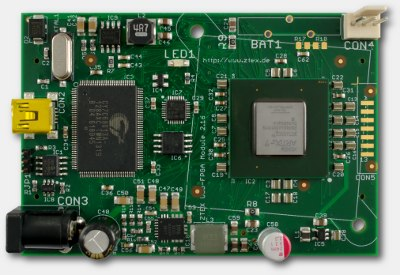
\includegraphics[width = 0.75\textwidth]{figures/fpga216.jpg}
	\caption{A ZTEX 2.16 FPGA board} 
	\label{fig:ztex}
\end{figure}

\Aref{fig:ztex} ábrán látható ZTEX panel mellett tettem le a voksom. A kártyán található egy USB-s loader, így JTAG programozó eszköz sem feltétlenül szükséges az FPGA feltöltéséshez, illetve FLASH memória is található az eszközön, így automatikusan minden indulákor betöltődik a firmware az FPGA-ba.


\begin{figure}[!ht]
	\centering
	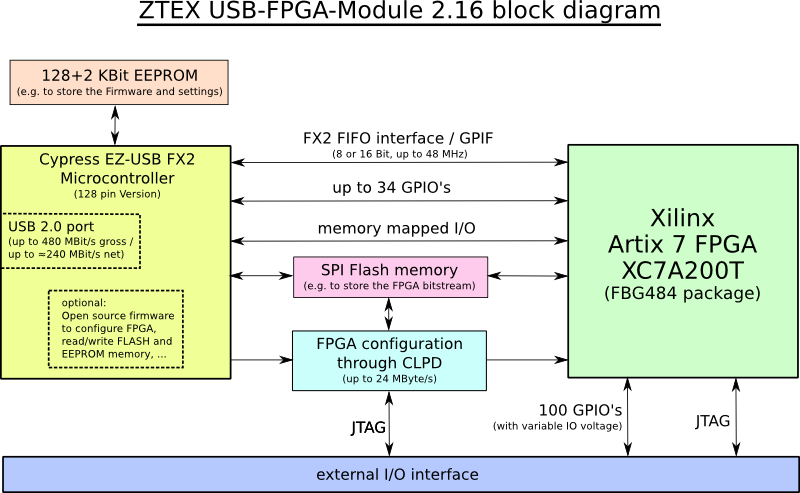
\includegraphics[width = 0.8\textwidth]{figures/usb-fpga-216.png}
	\caption{A ZTEX 2.16 FPGA board felépítése} 
	\label{fig:ztex_block}
\end{figure}

\todo[inline]{Képhiba}

Ezen felül a rajta található Xilinx Artix 7 FPGA megfelelő hűtését is biztosítja a panel. Az FPGA főbb datai \aref{table:artix7spec} táblázatban láthatóak. Ez az eszköz a Xilinx jelegelg kereskedelemi forgalomban kapható egyik zászlóshajója, amit bizonyít is a ZTEX panel 500 Eurós vételára.

\begin{table}[]
\centering
\begin{tabular}{ll}
Logikai cellák               & 215360 \\
Szeletek                     & 33650  \\
CLB Flip-flopok              & 269200 \\
Eloszott memória (kb)        & 2888   \\
Blokk RAM/FIFO (36 kb/darab) & 365    \\
Blokk RAM összesen (kb)      & 13140  \\
                             &        \\
                             &        \\
                             & 
  
\end{tabular}
\caption{A Xilinx Artix 7 XC7A200T}
\label{artix7spec}    
\end{table}

Bár a jelenlegi modell mindössze 10\%-át foglalja le a teljes hardwarenek, a későbbi bővülésre is hagy lehetőséget

\subsection{Szigma-Delta (\Sigma\Delta)\ átalakítók}

Az FPGA nem rendelkezik analóg kiementekkel, azonban a CCB számára elő kell állítani a normál működés során visszamért analóg jeleket, hiszen ebben relik a szimulátor lényege, a vezérlő elektronika szmszögéből nincsen különbség a valós hardware és a szimulátor között. A szigma delta átalakító nagyon nagy vonalakban egy órajel és egy fix impulzusszélességű négyszögjel, mely vagy logikai egy értéket, vagy logikai nulla értéket vesz fel az órajel minden felfutó (vagy lefutó) élére. Az így kialakult impulzusjel kitöltési tényezője egy hosszabb mintavételi ablakot tekintve arányos a bemeneti kódszóval. Ezek után a jelet egy az órajelnél sokkal kisebb vágási frekvenciájú aluláteresztő szűrűvel feldolgozva analóg jelet kapunk. A szigma delta átalakító további előnye a PWM kimenethez képest, hogy a kvantálái zajt nagyfrekvenciás tartományba tolja.\cite{artofelectronics}

Igen félrevezető névvel szokás "1 bites DA" átalakítónak is nevezni. A kifejezés egyszerűséget és alacsony teljesítményt sugall, ennek ellenére a megoldás rendkívül lineáris és nagy felbontású eredményt ad, így elterjedten használják pl. audio eszközökben is.

A mi esetünkben két részre bontható az átalakító. A modellben fut egy analógjelből digitális jelet létrehozó szigma-delta átalakító, majd az így kiadott digitális jelet szűrjük már az FPGA-n kívül egy aluláteresztő szűrűvel. \Aref{fig:sigmadelta} ábra szemlélteti az átalakító működését. A bejövő analalóg jelből levonjuk a hibajelet, majd egy komparátor összehasonlítja egy referenciával. Amennyiben nagyobb a bejövő jel, a kimenet logikai "1" értéket vesz fel, ha kisebb, logikai "0"-t. Ezt a jelet, egy 1-bites DAC-on keresztül vezetve akkumuláljuk, így kialakítva a hibajelet. 

\begin{figure}[!ht]
	\centering
	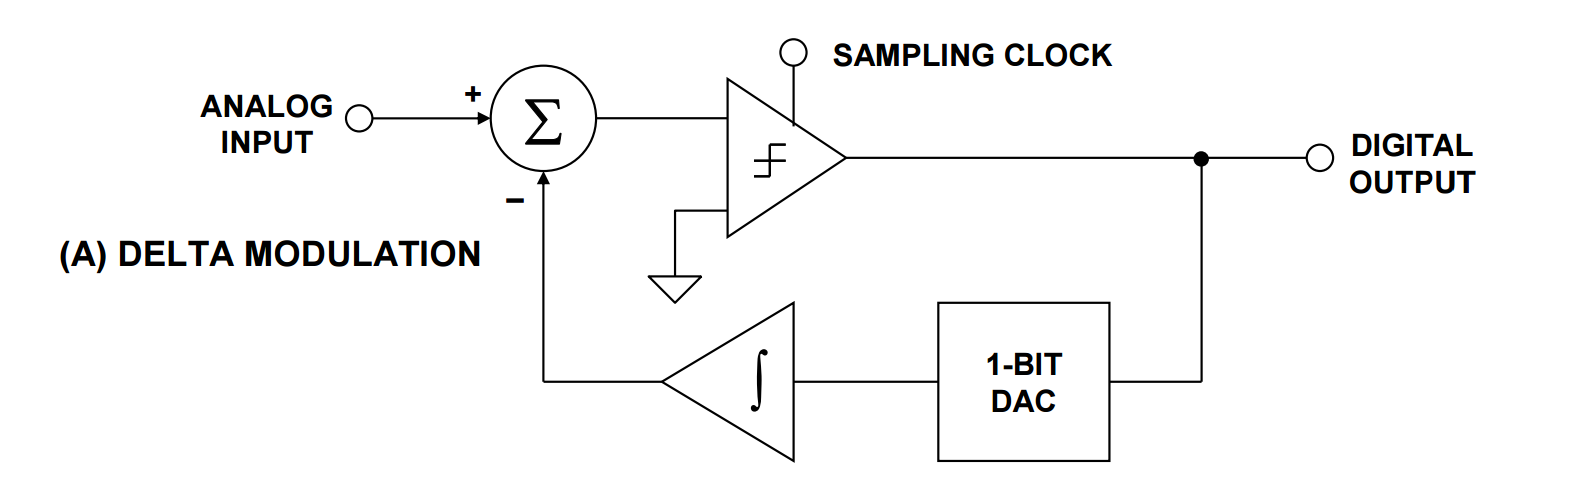
\includegraphics[width = 0.75\textwidth]{figures/sigmadelta.png}
	\caption{A szigma-delta átalakító} 
	\label{fig:sigmadelta}
\end{figure}

Az így kapott jelet már az FPGA lábára vezethetjük.

\begin{figure}[!ht]
	\centering
	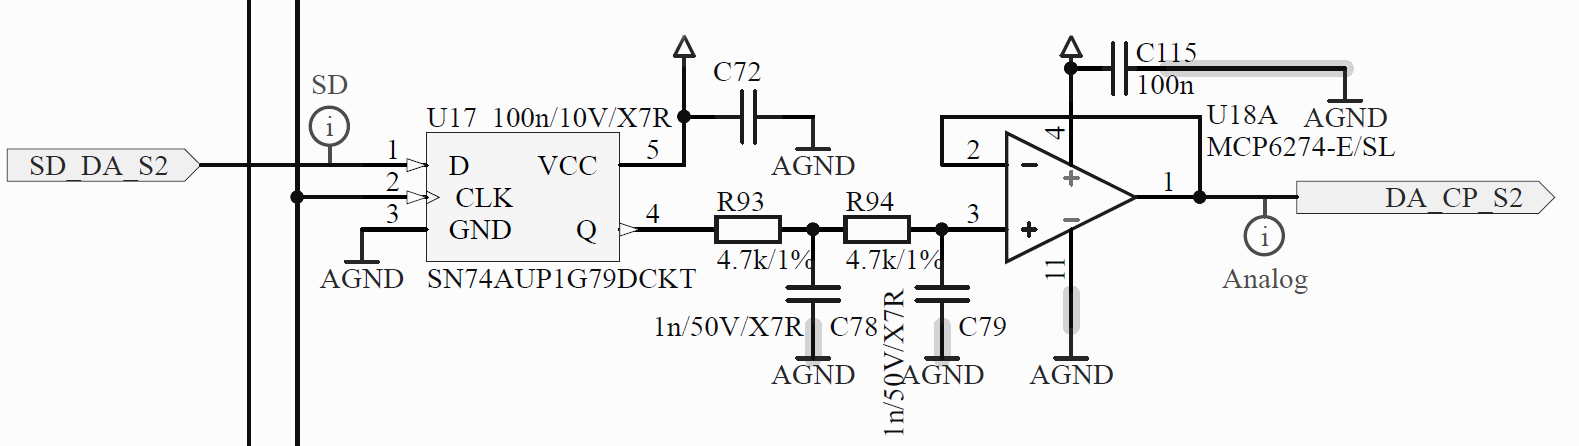
\includegraphics[width = \textwidth]{figures/lowpassfilter.png}
	\caption{A négyszögjelet fogadó aluláteresztő szűrő} 
	\label{fig:lowpass}
\end{figure}

\Aref{fig:lowpass} ábrán látható aluláteresztő szűrő kimenet már közvetlenül a CCB analóg bemenetére csatalkozik. A CCB analóg mérései differenciálisak a valóságban, mivel a valós enelktronikában sokkal nagyobb zaj éri a rendszert. A modellen azonban ez a zavar nem jelentős, így a mérés negatív jelét földre kötjük.



\section{Simulink modell}

A futtatandó modell magában foglalja a teljesítményelektronikai elemek modelljét, egy motor modellt és egy mechanikai terhelés modellt. Hiányossaág volt a modellnek, hogy a DC link feszültésge egy konstans érték volt, így a különböző terhelések DC feszültségre való visszahatásást nem lehetett vizsgálni. További hiányosság, hogy a hálózat paramétereit sem vette így figyelembe a modell.

\subsection{A rendelkezésre álló modell}

\subsection{Az implementál bemeneti modell}

\begin{figure}[]
	\centering
	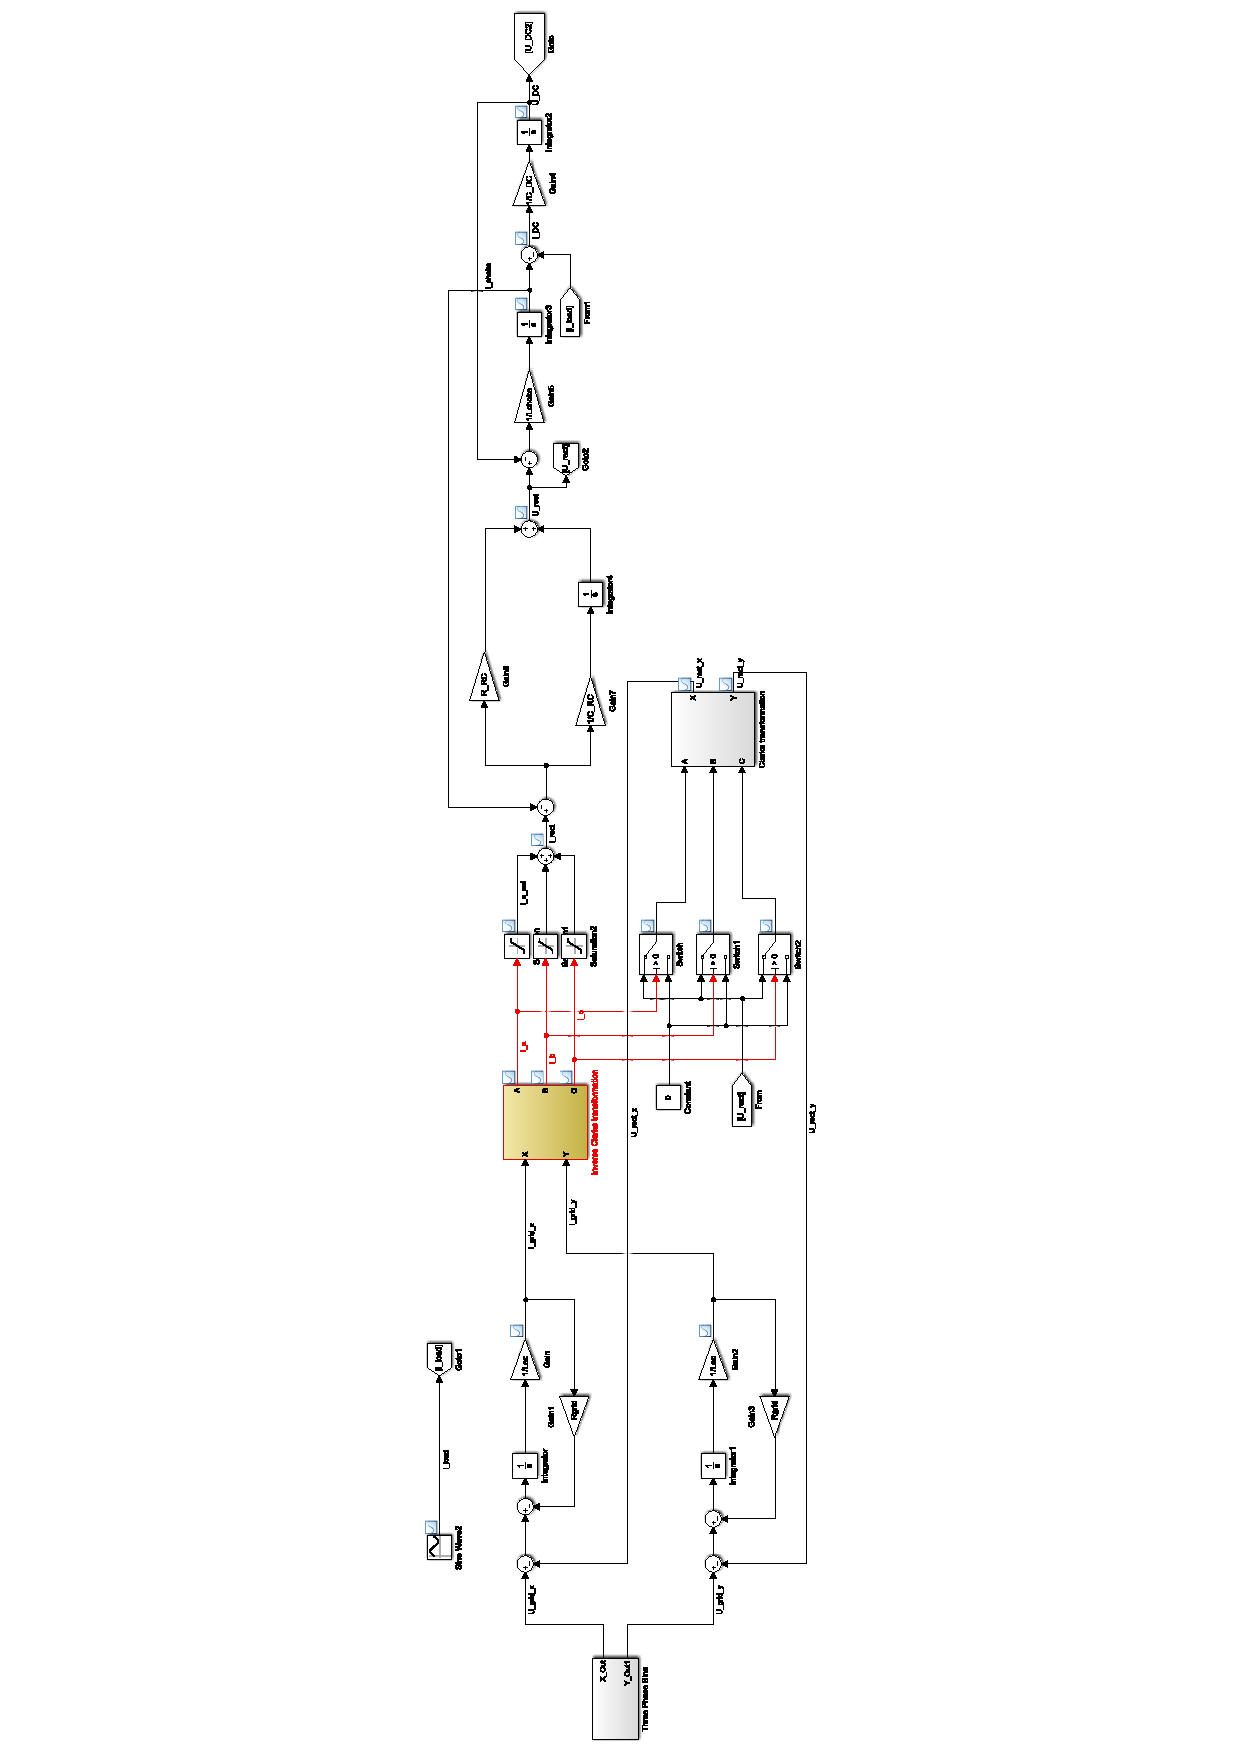
\includegraphics[width = \textwidth]{figures/model_continous.pdf}
	\caption{A frekvenciaváltó bemenetének folytonos modellje} 
	\label{fig:cont_input_model}
\end{figure}

A feladat tehát az volt, hogy a korábbi modellt egészítsem ki egy olyan blokkal ami a felsorolt hiányosságokat orvosolja. Az elkészítendő modellnek tartalmaznia kell tehát egy háromfázisú hálózatmodellt, a diódás hidat, a bemeneti DC folytót, illetve a DC link kondenzátort. A modellezendő főáramkori részt \aref{fig:input_marked} ábrán jelöltem. 

\begin{figure}[H!]
	\centering
	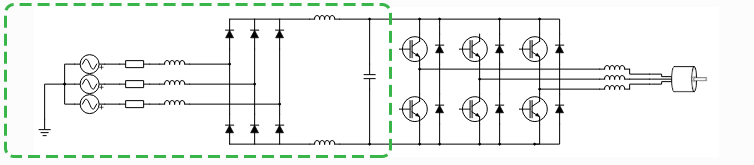
\includegraphics[width = \textwidth]{figures/VFDschematic_choke_marked.png}
	\caption{A frekvenciaváltó bemenetének folytonos modellje} 
	\label{fig:input_marked}
\end{figure}

A számítások megkönnyításe érdekében célszerű a háromfázisú hálózatot x-y komponensekkel reprezentálni.


\begin{equation}

\begin{bmatrix}
       U_a\\[0.3em]
       U_b\\[0.3em]
       U_c          
\end{bmatrix}
=
\begin{bmatrix}
       1 & 0      \\[0.3em]
       -\frac{1}{2} & \frac{sqrt{3}}{2}       \\[0.3em]
       -\frac{1}{2} & -\frac{sqrt{3}}{2}
\end{bmatrix}
\begin{bmatrix}
       U_x\\[0.3em]
       U_y         
\end{bmatrix}


\end{equation}

\begin{figure}[H!]
	\centering
	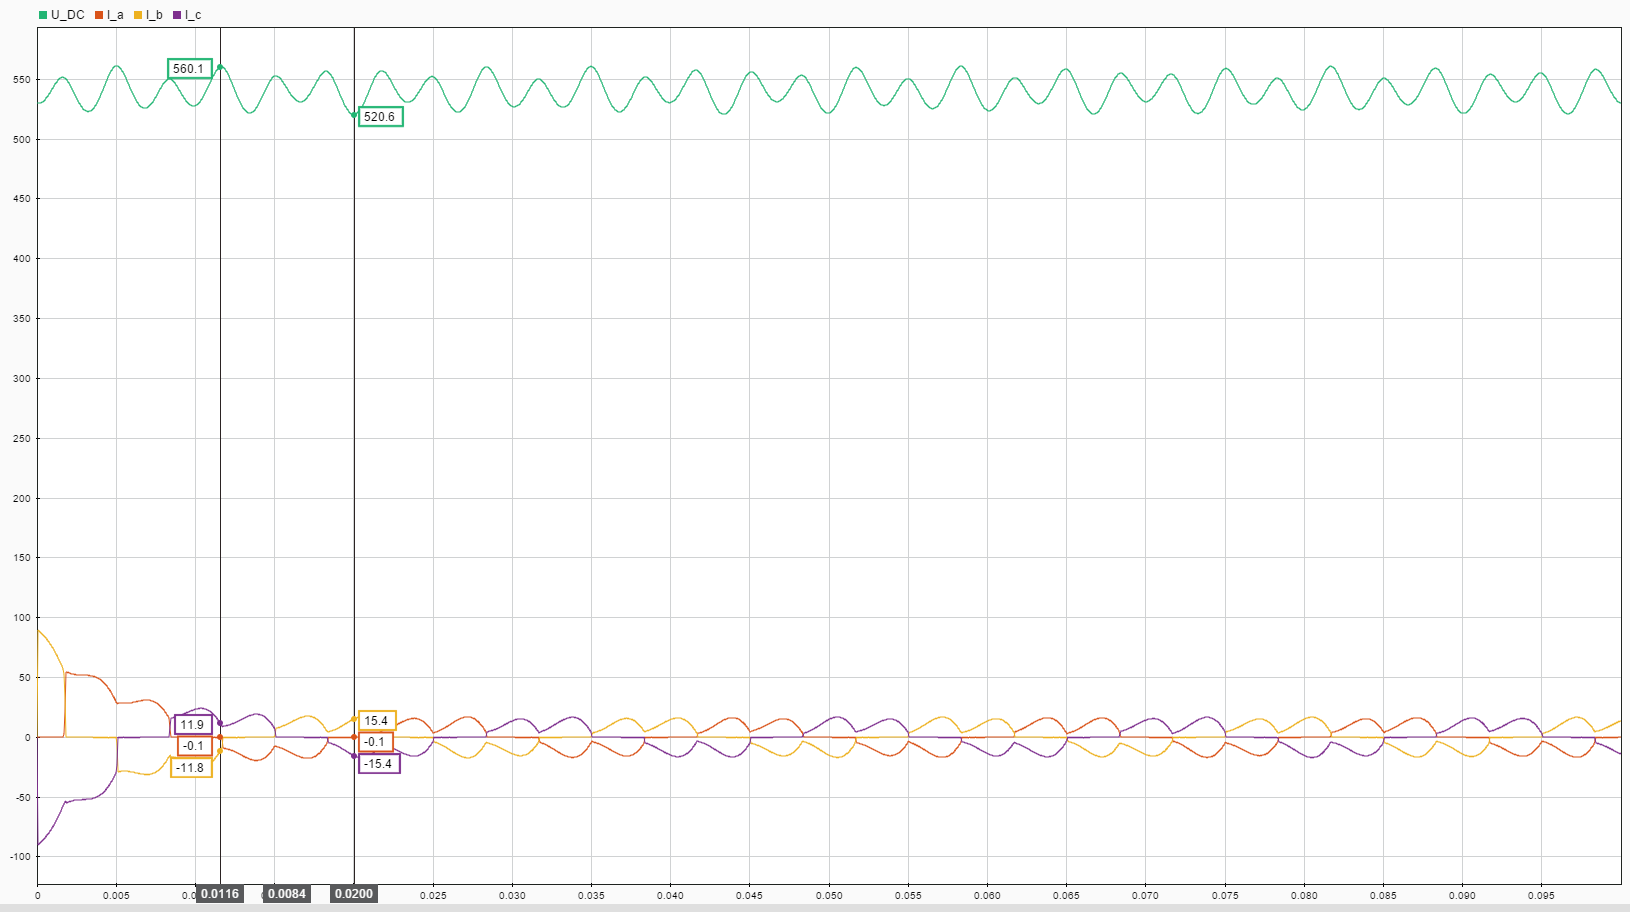
\includegraphics[width = \textwidth]{figures/continous_testrun_1.png}
	\caption{A folytonos modell szimulációja} 
	\label{fig:cont_run}
\end{figure}




\section{A szimulátor szerepe a folyamatban}
\section{A szimulátor felépítése}
\subsection{A hardware felépításe}
\subsection{A firmware felépítése}